%This work is licensed under the Creative Commons Attribution-NonCommercial-NoDerivs 3.0 United States License. To view a copy of this license, visit http://creativecommons.org/licenses/by-nc-nd/3.0/us/ or send a letter to Creative Commons, 444 Castro Street, Suite 900, Mountain View, California, 94041, USA.

\section{Introduction}

In the search for alternative mechanisms to reduce the intrinsic divergence of the electron beam upon photoemission, a possible area of interest was Plasmon-Assisted Photoemission (PAPE). 
This avenue of investigation was motivated by Zawadzka et al \cite{zawadzka_evanescent_2001} who indicate that when driving a surface plasmon on gold they witnessed a reduction in the emission angle of photoemitted electrons.
In their paper, the authors mount a gold foil on a prism; the laser is incident on the gold through the prism.
This geometry is called the Kretschmann geometry.

While this geometry is common, due to fears about the lack of heat conduction through the glass and the power needed to generate a sufficient electron beam current, that UEM applications should explore the ``grating coupling'' geometry.
In this geometry, the plasmon is driven on a periodic surface rather than a flat surface attached to glass.
Futher, in this geometry the back surface is now free to be attached to a heat sink.

\subsection{Driving the Plasmon}

Every material has an intrinsic plasma frequency given by 
\begin{equation}
  \omega_{P} = \sqrt{\frac{n e^2}{\varepsilon_{0} m^*}}
\end{equation}
where $n$ is the electron density and $m*$ is the effective mass of the material.
In order to drive a plasmon on the surface of a material, the portion of the laser wave-vector parallel to the plasmon ($k_{Lx}$) must be matched to the wave-vector of the surface plasmon.
\begin{equation}
  k_{P} = k_{Lx} + i k_{G}
\end{equation}


\section{Experimental Attempts}

\subsection{Commerical Grating on Glass}

For proof-of-concept purposes the first experiment was run on a commercially available gold foil on glass holographic grating.
Like the Kretschmann geometry, a foil on glass grating is vulnerable to heating problems; a plasmon creates a large amount of heat but the glass is a poor heat conductor.
The grating was operational as the angles were tuned attempting to drive the plasmon.
At the instant that the plasmon started, a bright flash was visible on the scintillator screen then disappeared.

After this, the grating showed signs of damage.
\ref{fig:grating-damage} shows the results of Scanning Electron Microscopy (SEM) on the grating.
The damage pattern is round and of the size of the laser spot used to drive the plasmon.
The extent of the damage indicates a large temperature increase, which given the other evidence of the test, can be assumed to be from the sudden appearance of a surface plasmon.

The most important result was that a plasmon was driven successfully; this created the heat that destroyed the grating.
Further this experiment validated the decision not to persue a Kretschmann geometry for fear of heat damage at these high powers.

\begin{figure}
  \centering
  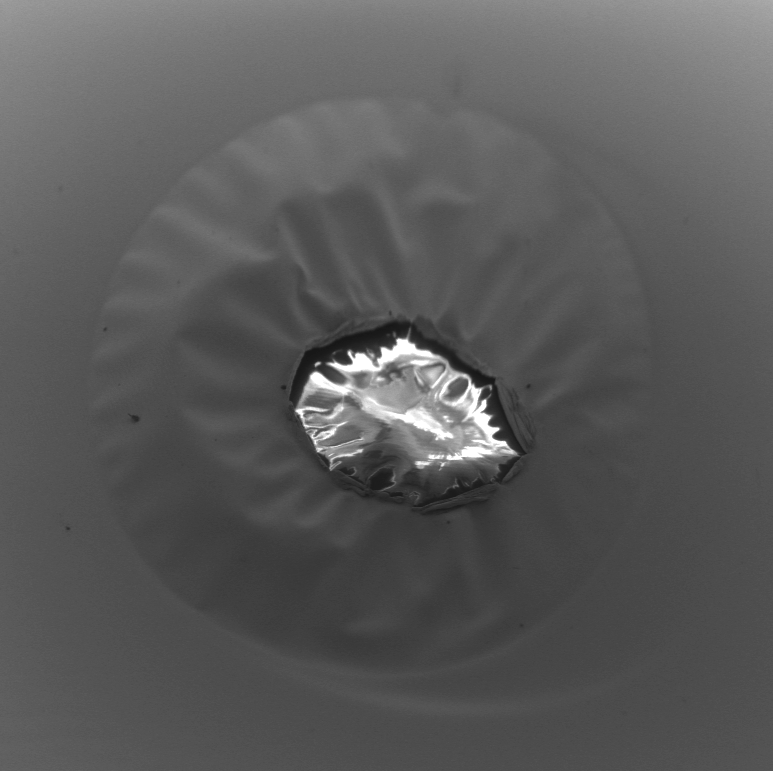
\includegraphics{damage.png}
  \caption{Damage to commerical gold-on-glass holographic grating.}
  \label{fig:grating-damage}
\end{figure}

\subsection{Sinusoidal Grating}

\subsection{Sinusoidal Grating, Rotated}

\subsection{Trenched Grating}
